\documentclass[border=8pt, multi, tikz]{standalone}
\usepackage{import}
\usepackage{graphicx}
\usetikzlibrary{shapes, arrows, 3d}
\subimport{../layers/}{init}
\def\input_image{../examples/output_image.png}

\begin{document}
	\begin{tikzpicture}
	\tikzstyle{fillwhite} = [fill=white,inner sep=0pt, opacity=1]
	\tikzstyle{connection}=[ultra thick,every node/.style={sloped,allow upside down},draw=\edgecolor,opacity=0.7]
% Generator	
	\pic[shift={(0, 0, 0)}] at (0,0,0)
	{SolidBox={
			name=generator,
			label=\LARGE Generator,
			fill=green,
			height=15,
			depth=15,
			opacity=0.1,
			width={20}
		}
	};
% Real Image
	\pic[shift={(-8, 0, 0)}] at (generator-west)
	{SolidBox={
		name=real_image,
		caption=\LARGE Real image,
		fill=white,
		height=15,
		depth=15,
		width={1}
		}
	};

	\draw [connection] (real_image-east) -- node [coordinate] (test) {} (generator-west);
	\path (test) -- node [fillwhite] {\midarrow} (generator-west); 
	
% Random Attributes	
	\node[shift={(0,-2,0)}, thick, rectangle, minimum height=1 cm, minimum width=1 cm, align=center] (random) at (test) {\large Random\\ \large attributes};
	\draw [connection] (random) |- node[fillwhite, near start] {\midarrow} (test);	

%	Real Images
	\pic[shift={(0, 11, 0)}] at (generator-north)
	{SolidBox={
		name=real_images,
		fill=white,
		height=15,
		depth=15,
		width={1,1}
	}
	};

	\pic[shift={(2, 0, 0)}] at (real_images-east)
	{SolidBox={
			name=real_images_2,
			fill=white,
			height=15,
			depth=15,
			width={1, 1}
		}
	};
	\path (real_images-east) -- node (real) {$\dots$} (real_images_2-west);
	\node [shift={(1.25,0,0)}, below] at (real_images-nearsouth) {\LARGE Real images};

	\pic[shift={(4, 0, 0)}] at (generator-east)
	{SolidBox={
		name=fake_image,
		fill=white,
		height=15,
		depth=15,
		width={1}
		}
	};
	\draw [connection] (generator-east) -- node [fillwhite] {\midarrow} (fake_image-west);

	\path (generator-northwest) -- node[coordinate, near start] (generator_north_1) {} (generator-northeast);
	\path (generator-northwest) -- node[coordinate, near end] (generator_north_2) {} (generator-northeast);
	\path (generator-nearsouthwest) -- node[coordinate, near start] (generator_south_1) {} (generator-nearsoutheast);
	\path (generator-nearsouthwest) -- node[coordinate, near end] (generator_south_2) {} (generator-nearsoutheast);		

% Attributes
\pic[shift={(2, 4.25, 0)}] at (real_image-north)
{SolidBox={
		name=attributes,
		label= Attribute \\ prediction,
		fill=yellow,
		height=5,
		depth=5,
		width={12}
	}
};

\path (real_image-north) |- node [coordinate] (dummy_0) {} (attributes-west);

\draw [connection] (real_image-north) -- (dummy_0) -- node [fillwhite] {\midarrow} (attributes-west);
\draw [connection] (dummy_0) ++(0,-1) -| node [fillwhite, near start, rotate=180] {\midarrow} (attributes-nearsouth);

% Segmentation
\pic[shift={(1, 6.75, 0)}] at (real_image-north)
{SolidBox={
		name=semantic_map,
		label= Semantic \\ segmentation,
		fill=orange,
		opacity=0.25,			
		height=5,
		depth=5,
		width={12}
	}
};
\node[canvas is zy plane at x=1.5, shift=({0,0,0}), inner sep=0] (image_0) at (semantic_map-east) {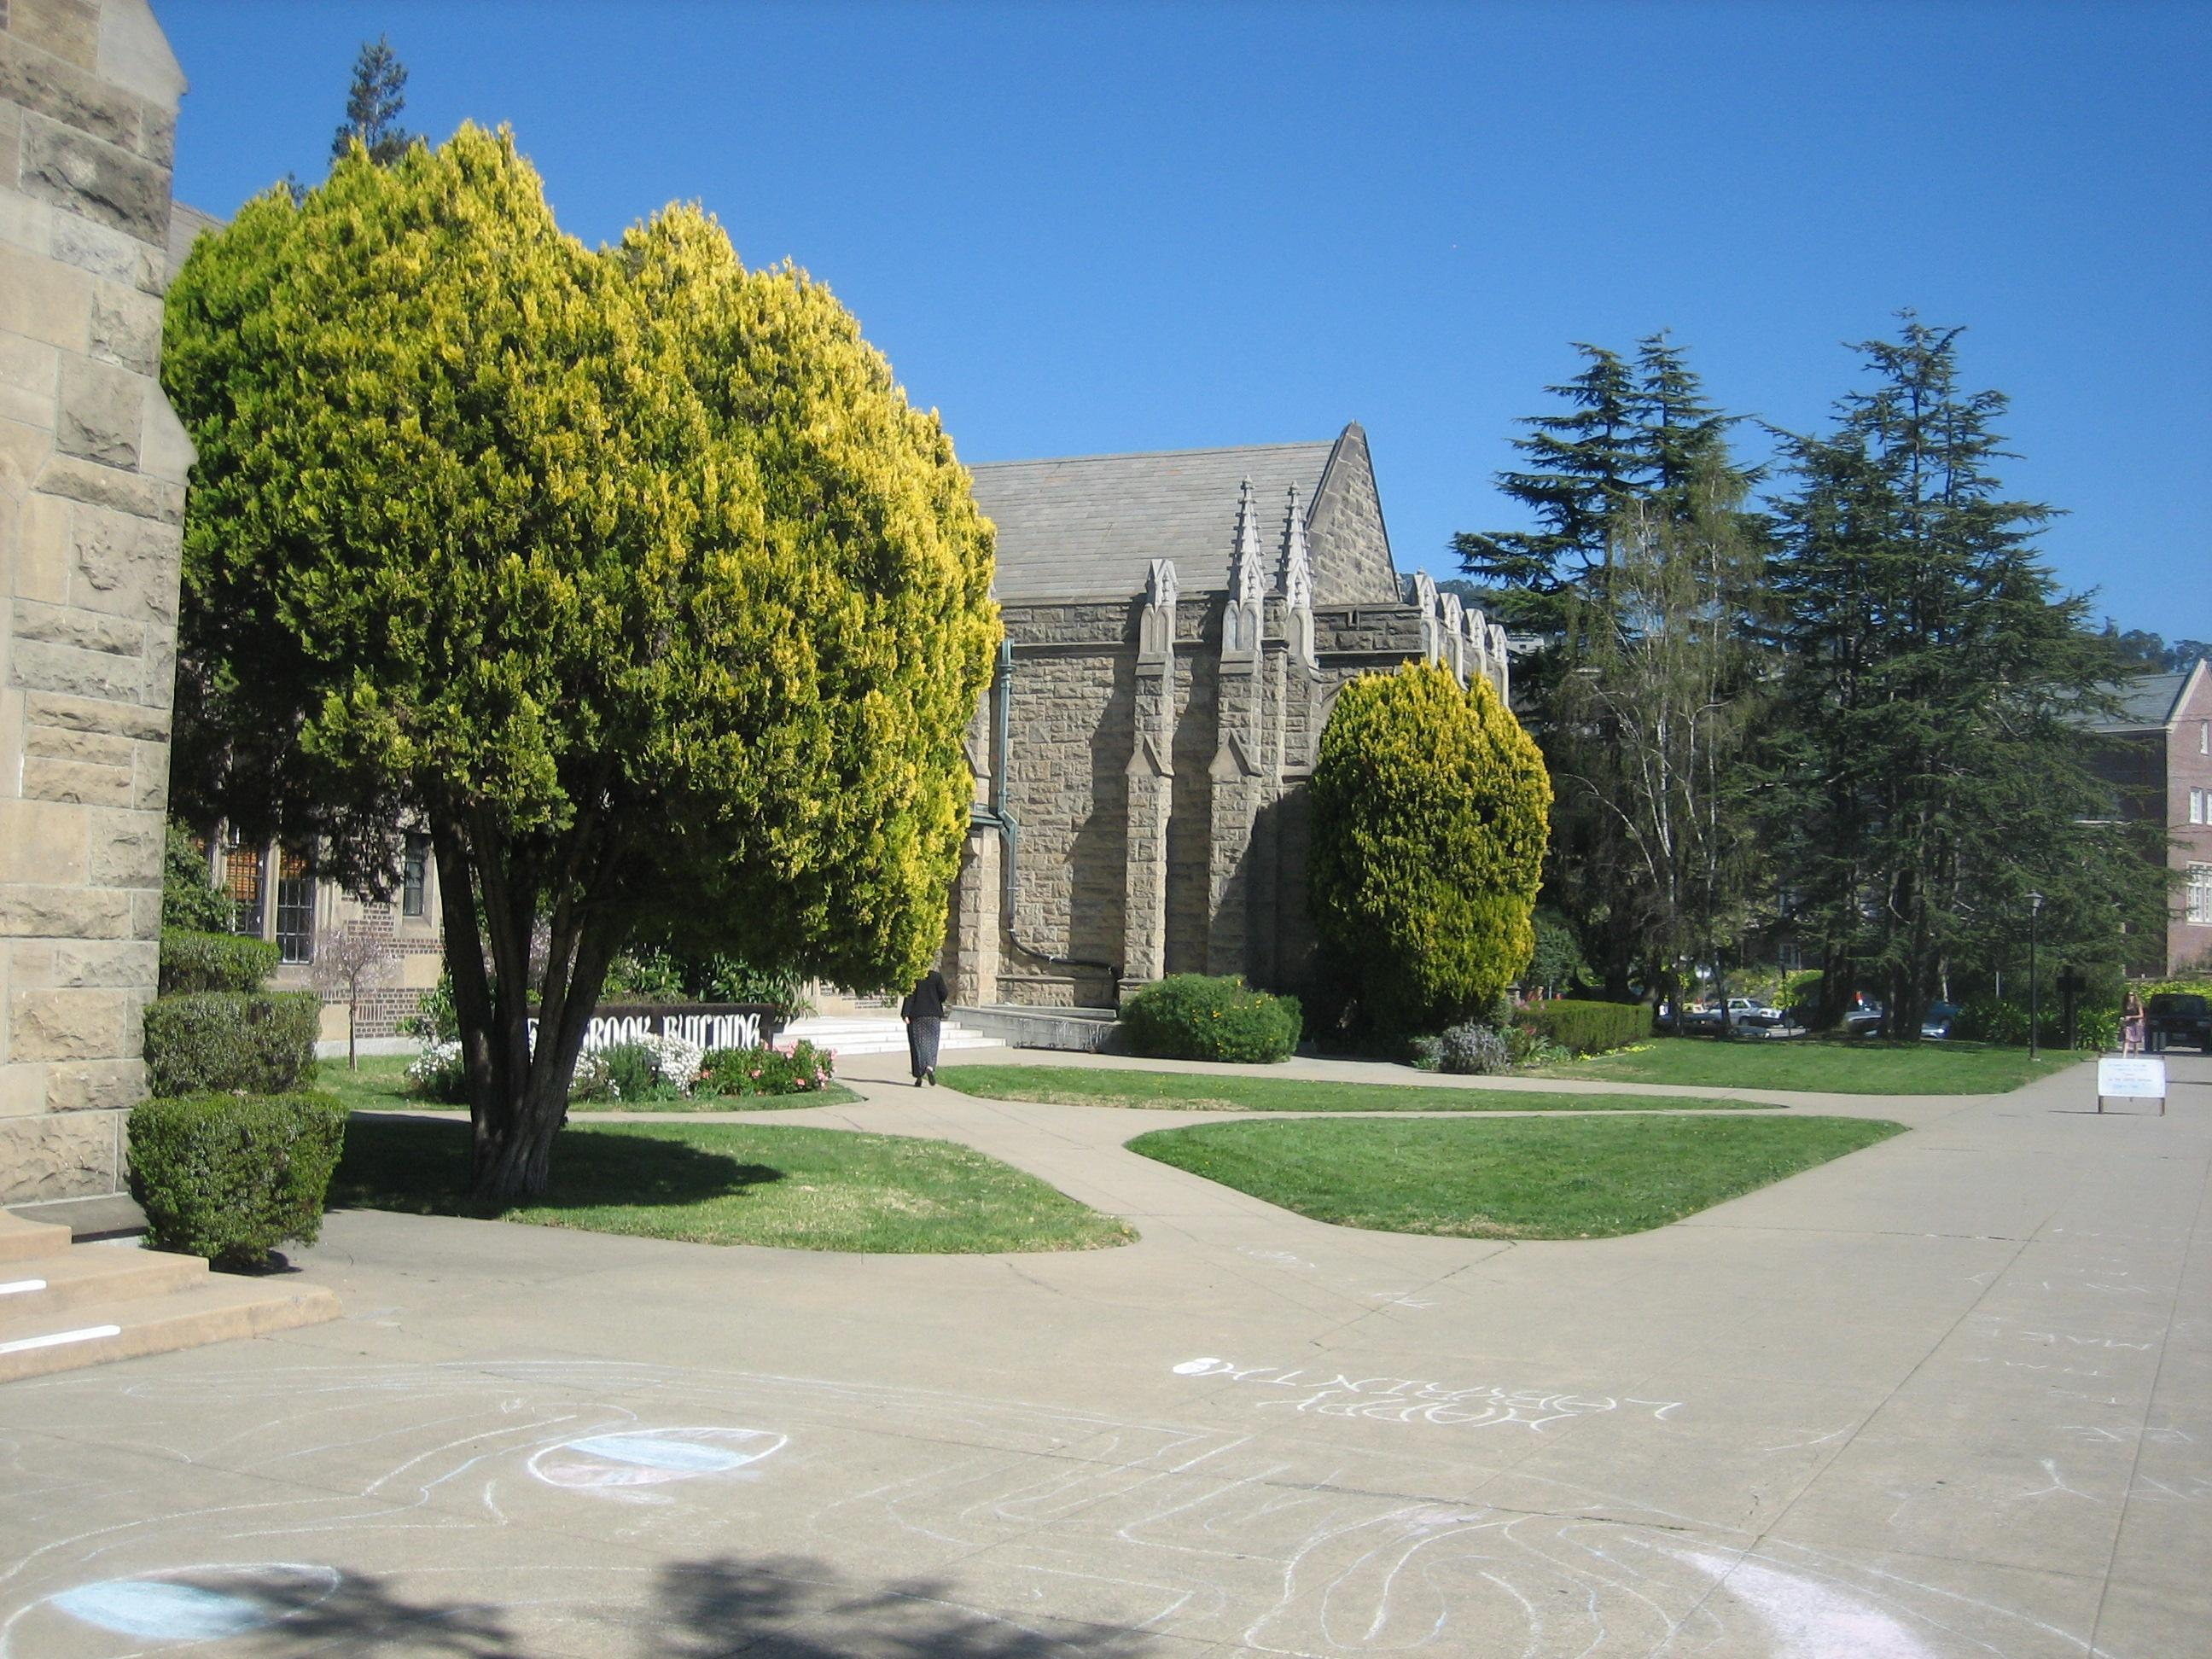
\includegraphics[width=2cm ,height=2cm ]{\input_image}};
\draw [connection] (semantic_map-east) --(image_0);				
\draw [connection] (dummy_0) |- node [pos=0.35, fillwhite] {\midarrow} (semantic_map-west);
\draw [connection] (dummy_0) ++(0,1) -| node [fillwhite, near start, rotate=180] {\midarrow} (image_0.south);

% Attribute Loss
	\pic[shift={(-3.5, -3.5, 0)}] at (fake_image-south)
	{SolidBox={
			name=attributes_2,
			label= Attribute \\ prediction,
			fill=yellow,
			height=5,
			depth=5,
			width={12}
		}
	};
	\draw [connection] (fake_image-south) |- node [near start, fillwhite] {\midarrow} (attributes_2-east);	
	\path (attributes_2-west) -| node[fillwhite, align=center] (att_loss) {\Large\textit{Attribute}\\\Large\textit{loss}} (generator_south_2);
	\draw [connection] (attributes_2-west) -- node [fillwhite] {\midarrow} (att_loss);
	\draw [connection] (random) |- node [near start, fillwhite] {\midarrow} (att_loss);
	\draw [connection, densely dashed] (att_loss) -- node [fillwhite] {\midarrow}(generator_south_2);

% Semantic Loss
	\pic[shift={(-1, 6.75, 0)}] at (fake_image-north)
	{SolidBox={
			name=semantic_map_2,
			label= Semantic \\ segmentation,
			fill=orange,
			opacity=0.25,	
			height=5,
			depth=5,
			width={12}
		}
	};

	\node[canvas is zy plane at x=-2, shift=({0,0,0})] (image_1) at (semantic_map_2-west) {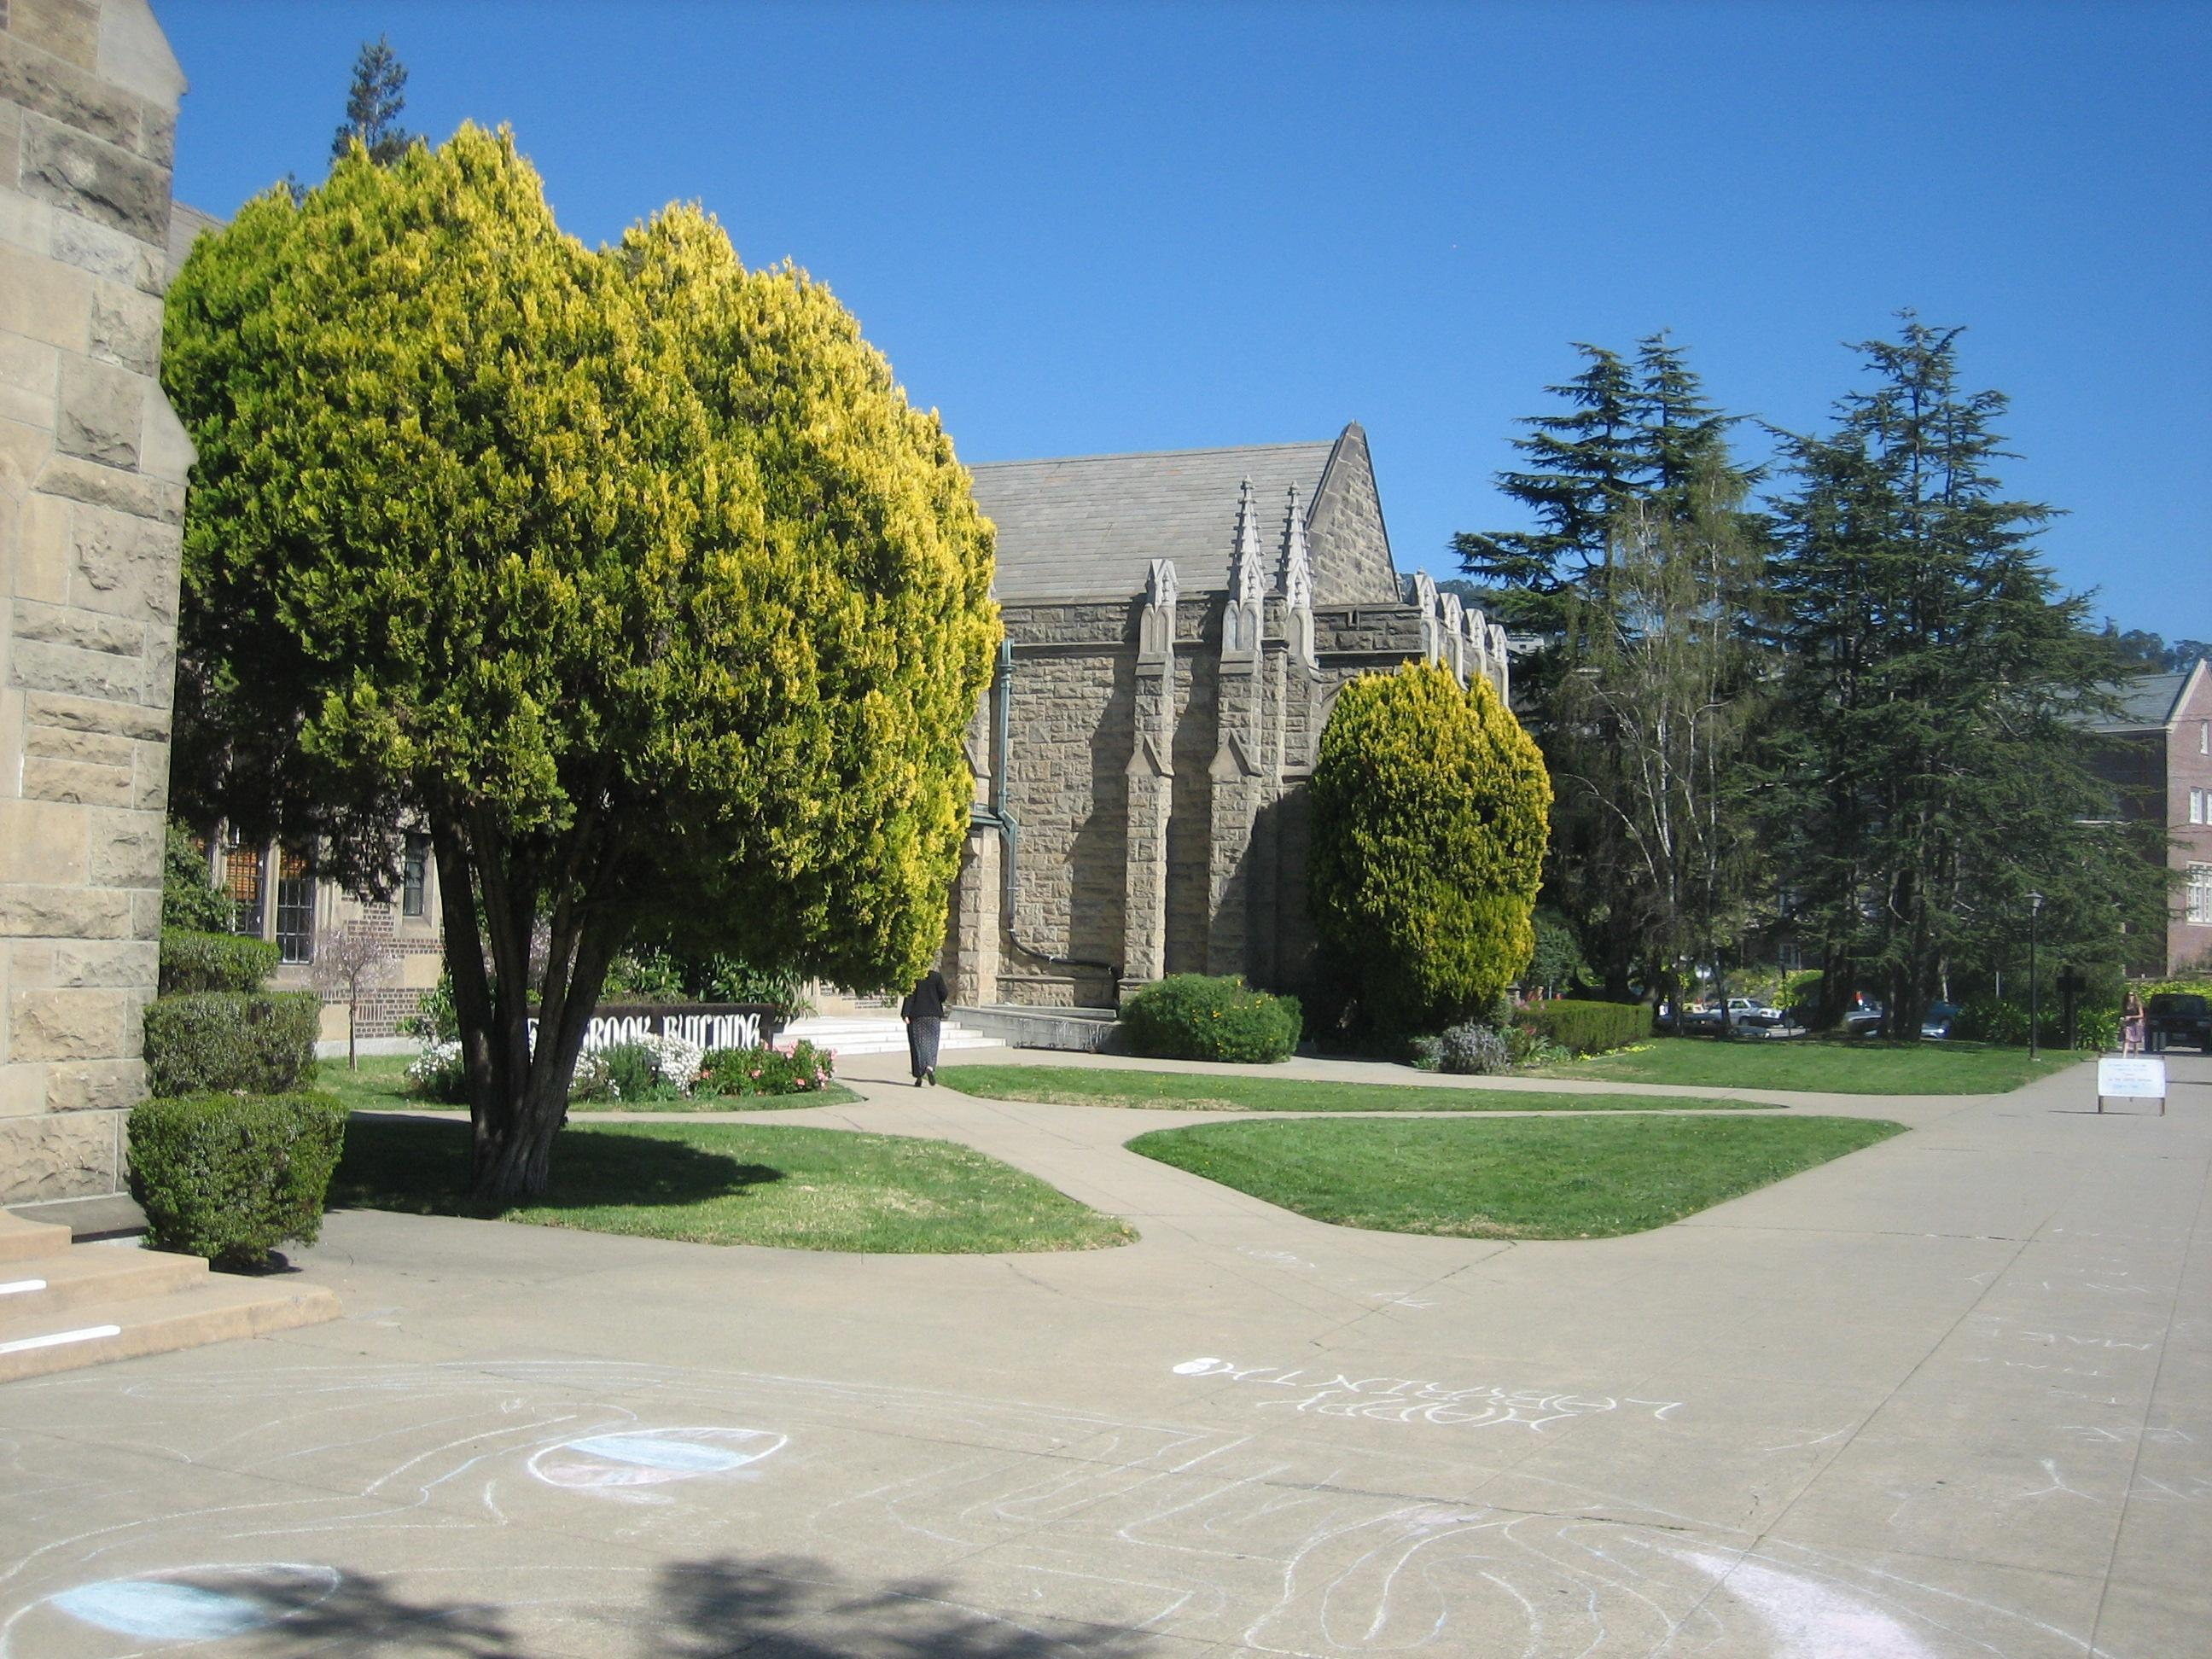
\includegraphics[width=2cm ,height=2cm ]{\input_image}};		
	\draw [connection] (fake_image-north) -- node[fillwhite] {\midarrow} (semantic_map_2-nearsouth);
	\path (semantic_map_2-west) -| node[fillwhite, align=center] (sem_loss) {\Large\textit{Semantic}\\ \Large\textit{loss}} (generator_north_1);
	\draw [connection] (image_0) --  node[fillwhite] {\midarrow} (sem_loss);				
	\draw [connection] (semantic_map_2-west)  --(image_1) -- node[fillwhite] {\midarrow}(sem_loss);
	\draw [connection, densely dashed] (sem_loss) -- node[near end, fillwhite] {\midarrow} (generator_north_1);


%Cycle consistency Loss	
	\draw [connection] (fake_image-northwest) -- node [inner sep=0, fillwhite] (rec) {\midarrow} (generator-northeast);
	\draw [connection] (attributes-east) -| node [pos=0.3, fillwhite] {\midarrow} (rec);
	

	\pic[shift={(-8, 0, -4)}] at (generator-farnorth)
	{SolidBox={
			name=rec_image,
			fill=white,
			height=10,
			depth=10,
			width={1}
		}
	};
	\draw [connection] (generator-farnorth) -- node [fillwhite] {\midarrow} ++(0,0,-4) -| node [fillwhite] {} (rec_image-west);
	\path (real_image-far) -- node [align=center] (cycle_loss) {\Large\textit{Cycle}\\\Large\textit{loss}} ++(0.5,0,-4.9);
	\draw [connection, dashed] (cycle_loss) -- node [fillwhite] {\midarrow} (generator-northwest);
	\draw [connection] (real_image-far) -- node [fillwhite, at end] {\midarrow} (cycle_loss.south west);
	\draw [connection] (rec_image-near) -- node [fillwhite] {\midarrow} (cycle_loss);
	\node [align=right, below left, inner sep=15] () at (rec_image-northwest) {\large Reconstructed \\ \large image};
	
% Discriminator
	\pic[shift={(5, 1, 0)}] at (fake_image-north)	
	{SolidBox={
			name=discriminator,
			label=\LARGE Discriminator,
			fill=red,
			height=15,
			depth=15,
			width={20},
			opacity=0.1
		}
	};	

	\node (dummy) [shift={(-2.5,0,0)}, inner sep=15] at (discriminator-west) {};

	\draw [connection] (fake_image-east) -| (dummy);
	
	\draw [connection] (real_images_2-east) -| (dummy) -- node [fillwhite] {\midarrow} (discriminator-west);
	
	\draw [connection] (dummy.south) -- (dummy.east);
	\draw[ultra thick, draw=\edgecolor, <->, >=latex', shorten >= 3pt, shorten <= 3pt] (dummy.south) to [bend left](dummy.north);
	\node[fill=\edgecolor, inner sep=2, circle] at (dummy.south) {};  
	\node[fill=\edgecolor, fill, inner sep=2, circle] at (dummy.north) {};  
	\node[fill=\edgecolor, fill, inner sep=2, circle] at (dummy.east) {};  
	
	
	\node (real) [shift={(2,0.5,0)}, inner sep=0] at (discriminator-east) {\Large Real};
	\node (fake) [shift={(2,-0.5,0)}, inner sep=0] at (discriminator-east) {\Large Fake};
	\draw [connection] (discriminator-east) ++(0,0.5) -- ++(1,0) |- (real);
	\draw [connection] (discriminator-east) ++(0,-0.5) -- ++(1,0) |- (fake);
	\node [draw, diamond, thick, shift={(5,0,0)}, inner sep=1] (correct) at (discriminator-east) {\Large Correct?};
	\draw [connection] (correct.west) -- ++(-0.25,0)  node [coordinate] (dummy_2) {} |- (real.east) ;
	\draw [connection] (fake) -| (dummy_2);
	
	\draw [connection, dashed] (correct) -- ++(2,0) -- node [fillwhite, rotate=90, near start, inner sep=2] {\large no} ++(0,-1) -- node [fillwhite] {\midarrow} ++(0,-4)  |- node [fill=white, opacity=1, near end, rotate=180] {\Large\textit{Discriminator loss}} ++(-9,0) -| node [near end, fillwhite] {\midarrow} (discriminator-nearsouth);
	
	\draw [connection, dashed] (correct) ++(2,0) -- ++(1,0) -- node [fillwhite, rotate=90, pos=0.3, inner sep=2] {\large yes} ++(0,-1) -- node [fillwhite] {\midarrow} ++(0,-8) |- node [fill=white, opacity=1, rotate=180, near end] {\Large\textit{Generator loss}} ++(-20,0) -| node [near end, fillwhite] {\midarrow} (generator_south_1);

  	\node [fillwhite, align=center, inner sep=2] (test2) [below] at (fake_image-nearsouth) {\LARGE Generated image};
	\end{tikzpicture}
\end{document}